\documentclass[12pt,a4paper,titlepage]{article}
\usepackage[scale=0.85]{geometry}
\usepackage[T1]{fontenc}
\usepackage[utf8]{inputenc}
\usepackage{graphicx}
\usepackage[french]{babel}
\restoreparindent
\graphicspath{ {images/} }
\usepackage{xcolor}
\usepackage{listings}
\usepackage{enumitem}
\usepackage{float}
\usepackage{appendix}

\definecolor{codegreen}{rgb}{0,0.6,0}
\definecolor{codegray}{rgb}{0.5,0.5,0.5}
\definecolor{codepurple}{rgb}{0.58,0,0.82}

\lstdefinestyle{mystyle}{
    backgroundcolor=\color{white},   
    commentstyle=\color{codegreen},
    keywordstyle=\color{magenta},
    numberstyle=\tiny\color{codegray},
    stringstyle=\color{codepurple},
    basicstyle=\ttfamily\footnotesize,
    breakatwhitespace=false,         
    breaklines=true,                 
    captionpos=b,                    
    keepspaces=true,                 
    numbers=left,                    
    numbersep=5pt,                  
    showspaces=false,                
    showstringspaces=false,
    showtabs=false,                  
    tabsize=2
}

\lstset{style=mystyle}

\title{Analyse Spectrale : travaux pratiques}
\author{Yassine Jamoud, Samy Haffoudhi}
\date{\today}

\begin{document}

\maketitle

\section{Détection d'oscillations}

\subsection*{Signal 1}

\subsection*{Signal 2}

\subsection*{Signal 3}

\subsection*{Signal 4}

\subsection*{Résumé des avantages et limites de chaque méthode}

\section{Détection d'exoplanètes par analyse spectrale de série temporelle}

\begin{enumerate}

    \item[1.] 
        Représentons la transformée de fourier en module de la fenêtre d'observation :

        \begin{figure}[H]
            \caption{Fenêtre d'observation}
            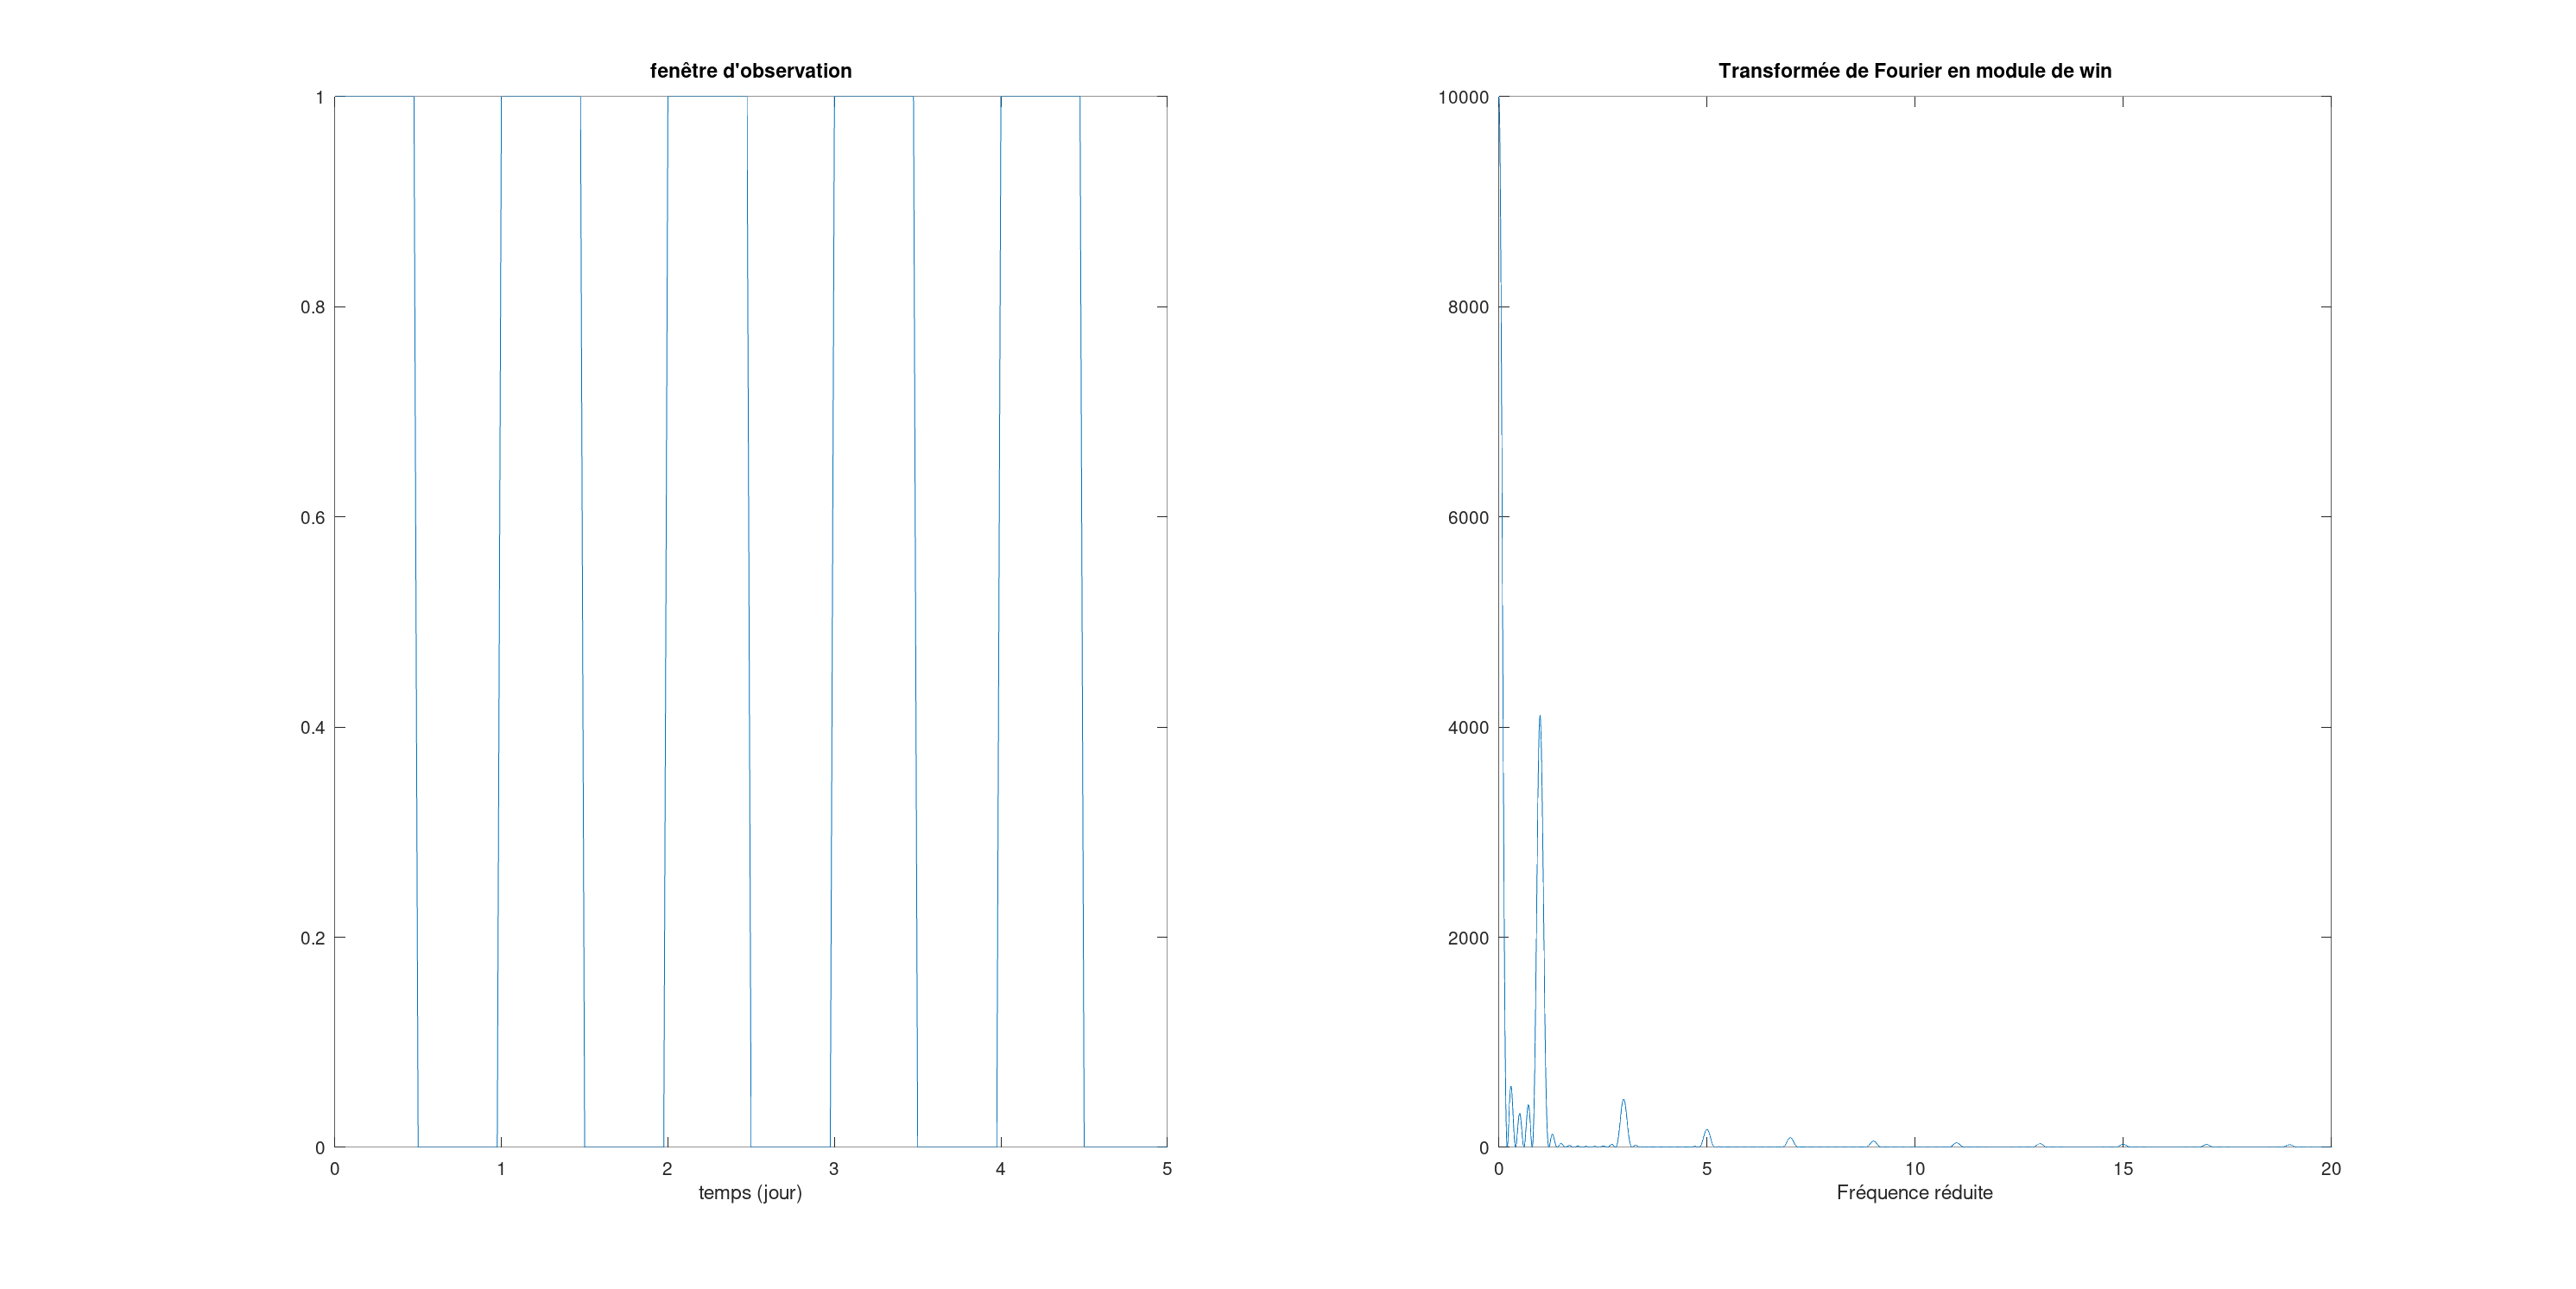
\includegraphics[width=\textwidth]{win}
            \centering
        \end{figure}

    \item[2.] 
        Représentons lle périodogramme du signal :

        \begin{figure}[H]
            \caption{Signal (données disponibles}
            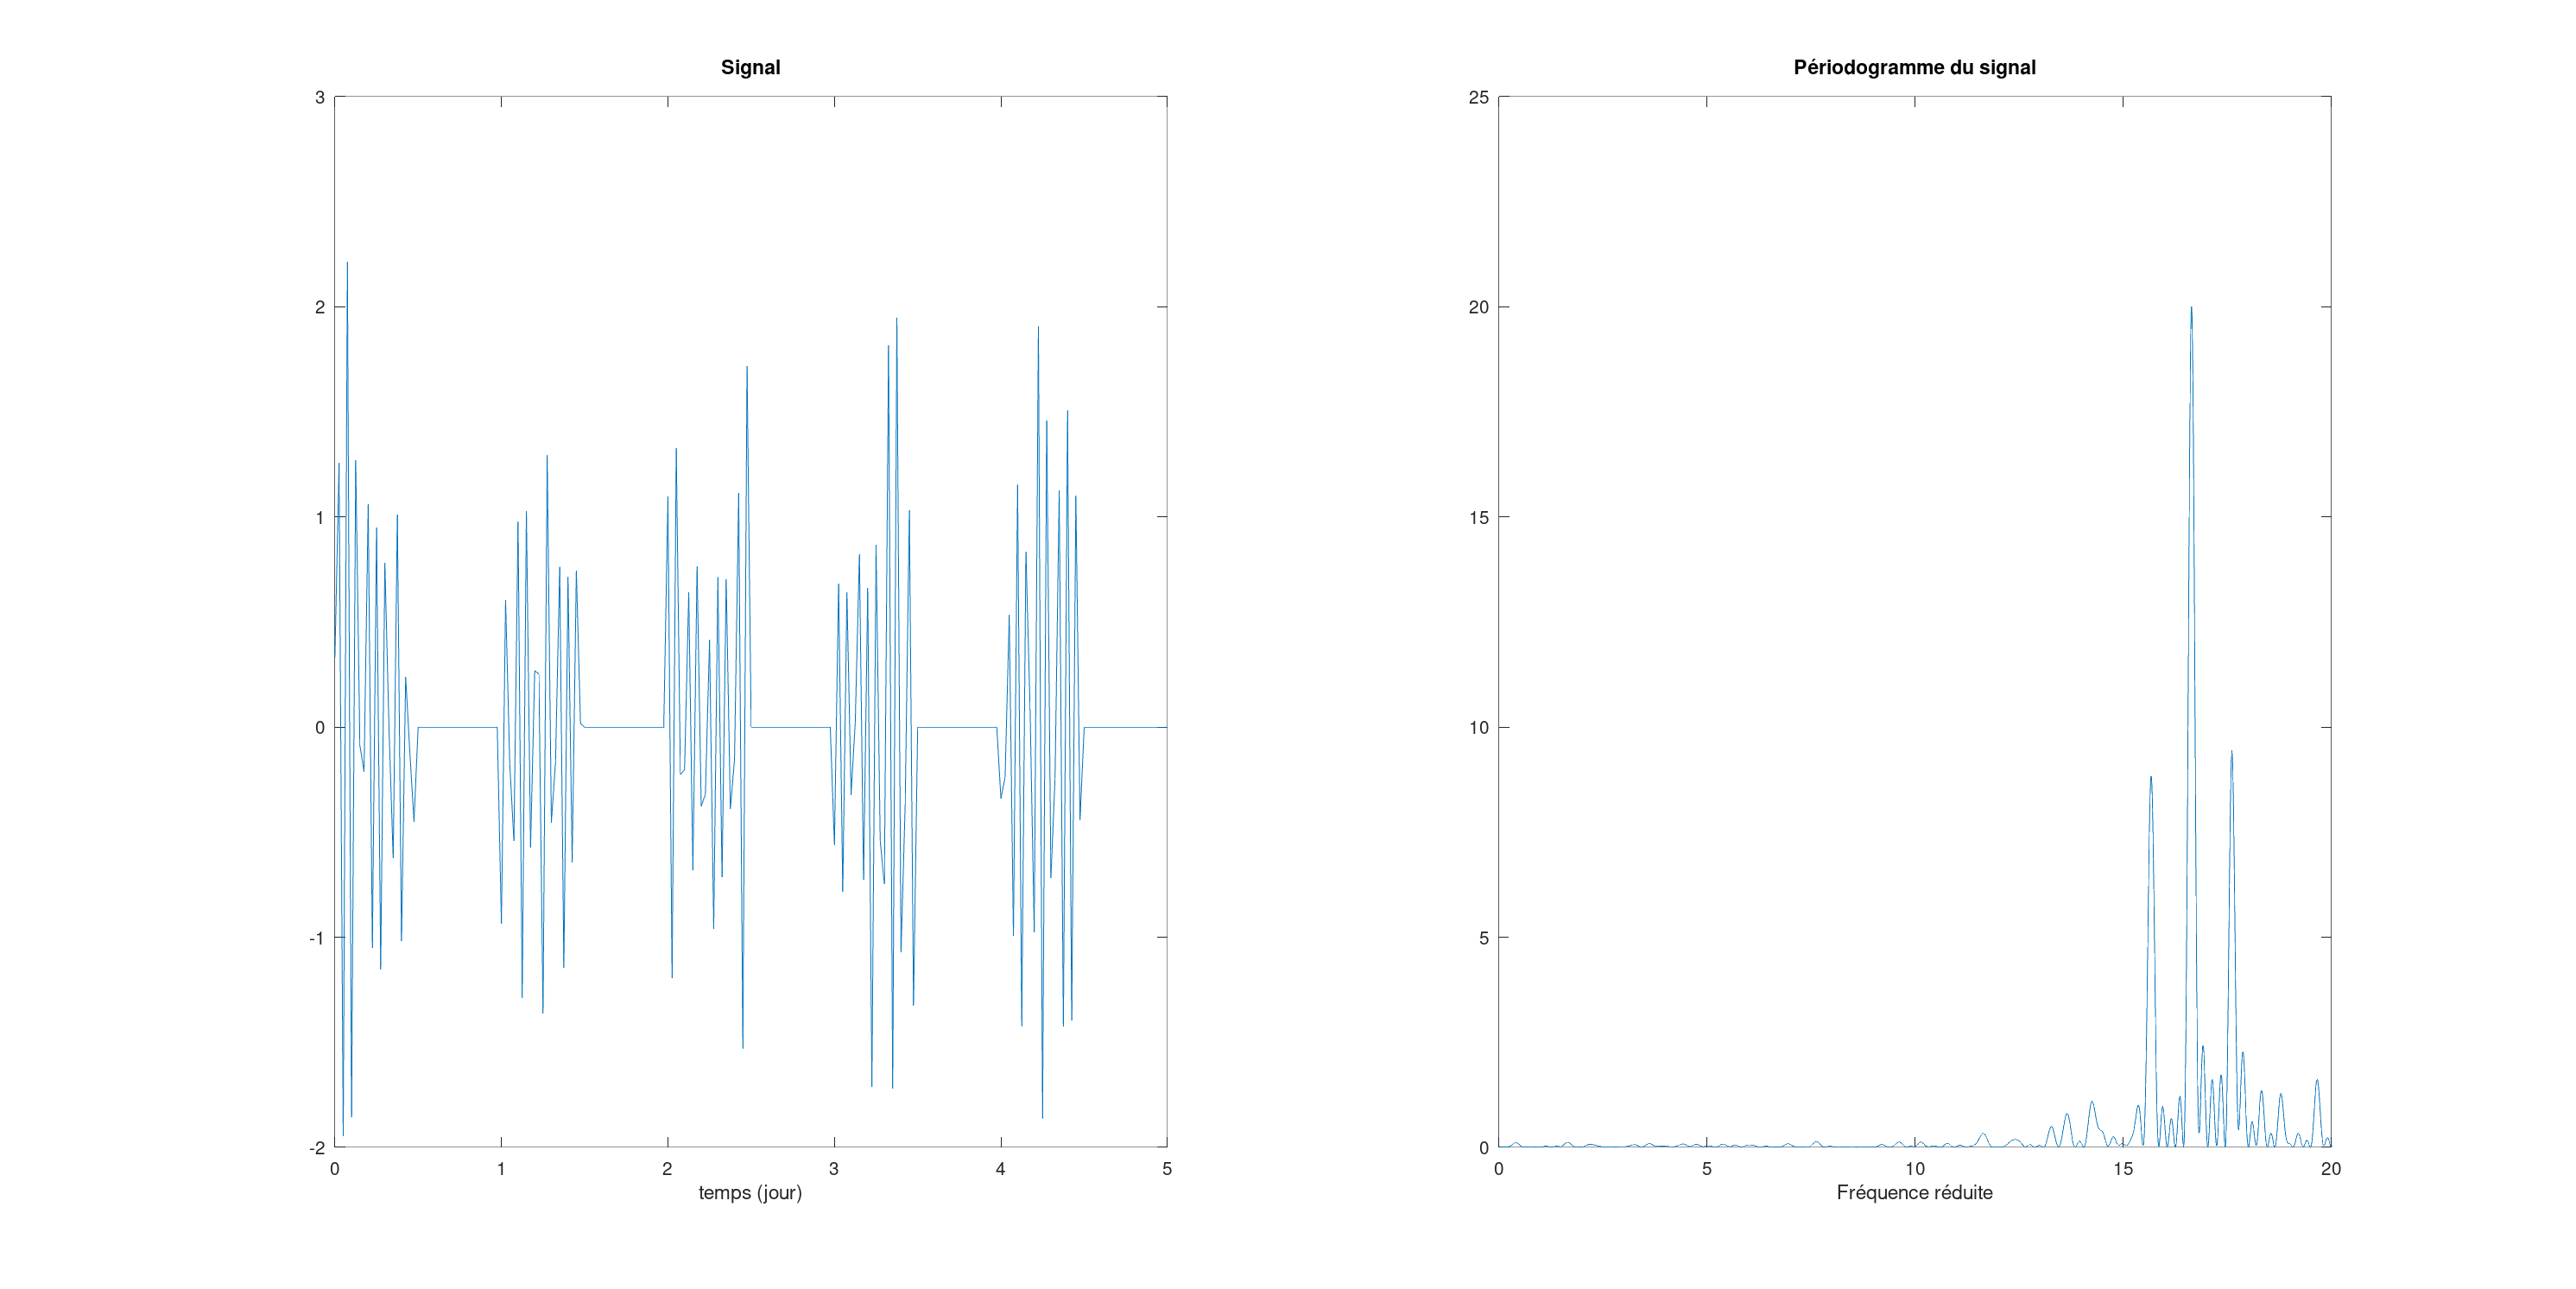
\includegraphics[width=\textwidth]{periodogramme_sig}
            \centering
        \end{figure}

    \item[3.] 

    \item[4.] 

\end{enumerate}

\begin{appendices}

    \section{Code Exercice 2}

\lstinputlisting[language=Matlab]{../astro.m}

\end{appendices}

\end{document}
